\documentclass[./\jobname.tex]{subfiles}
\begin{document}
%
\chapter{Siebensegmentanzeige}
%
\section{Einleitung}
%
In der ersten Aufgabe soll eine Siebensegmentanzeige mit Verilog implementiert werden. Die Anforderungen sind:
\begin{itemize}
	\item die Binärzahl korrekt den Ausgängen zuweisen (\enquote{hex}).
	\item \enquote{hex\_n} ist die negierte Version von \enquote{hex}\footnote{Ist hilfreich für\enquote{active low} Anzeigen.}.
	\item Die Zahlen 10 bis 15 nicht vergessen!
\end{itemize}
%
Zusätzlich zu den Anforderungen muss die Implementierung getestet und verifiziert werden. Dies bedeutet, dass alle Eingänge stimuliert und alle Signale im \enquote{Wave Window} angezeigt werden. Außerdem sollte der aktuelle Zustand der Ein- und Ausgänge als Lookup-Tabelle in der Modelsim-Konsole (\enquote{Transkript-Fenster}) angezeigt werden.
%
\section{Implementierung}
%
Für die Implementierung wurde die Verhaltensbeschreibung verwendet, da die \enquote{Gate-Primitive} nicht empfohlen wurde und die kontinuierliche Zuweisung zu umständlich wäre. Der Code kann in \autoref{lst:sevenseg} nachgelesen werden.
%
\lstinputlisting[language=Verilog,label={lst:sevenseg}, caption=Implementierung]{./code/sevenseg/src/sevenseg.sv}
%
\section{Test Bench}
%
Das Testkonzept ist eine for-Schleife, die abhängig von der Bit-Länge bis zum Maximum iteriert, siehe Codezeile \ref{code:bitsLength} in \autoref{lst:sim_tb_sevenseg}. Die Iterationsvariable wird in jedem Iterationsschritt \enquote{bin} zugewiesen. Dabei wird die tatsächliche Anzahl der Ein- und Ausgänge in binärer Darstellung im \enquote{Transcript} der Modelsim-Software dargestellt. Darüber hinaus wird die Siebensegmentanzeige im \enquote{Transcript} simuliert, siehe Codezeile \ref{code:startPlot} bis \ref{code:endPlot}.
%
\lstinputlisting[language=Verilog,label={lst:tb_sevenseg}, caption=Testbench für die Siebensegmentanzeige]{./code/sevenseg/sim/tb_sevenseg.sv}
%
\section{Simulationsscript}
%
In \autoref{lst:sim_tb_sevenseg} ist das Simulationsscript dargestellt. Es beinhaltet dieselben Befehle wie in der letzten Lehrveranstaltung, natürlich angepasst an die Siebensegmentanzeige.
%
\lstinputlisting[language=tcl,label={lst:sim_tb_sevenseg}, caption=Simulationsscript]{./code/sevenseg/sim/sim_tb_sevenseg.tcl}
%
\section{Transkript und Waveform Window}
%
In \autoref{fig: wavewindow.PNG} können die Ausgänge \enquote{hex} und \enquote{hex\_n} im Wavefomr Window überprüft werden. In \cref{ausgabeA,ausgabeB,ausgabeC,ausgabeD} ist der Commandline Output abgebildet, welcher ebenfalls zeigt, dass der Test erfolgreich war. 
%
\begin{figure}[H]
	\centering
	\noindent\adjustbox{max width=\textwidth}{%falls größer als \textwidth, wird das Bild verkleinert
		%trim option's parameter order: left bottom right top
		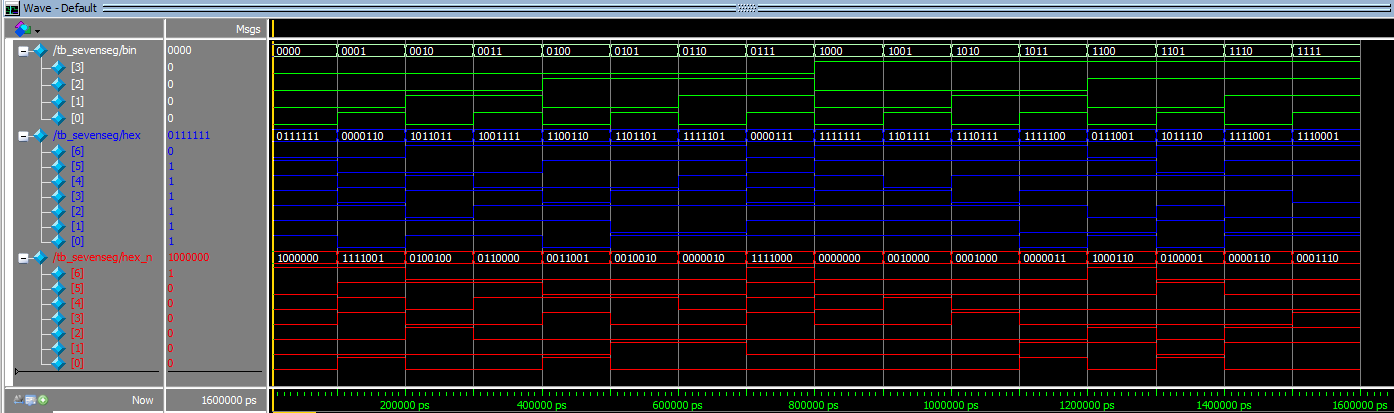
\includegraphics[width=1\textwidth]{./code/sevenseg/doc/wavewindow.PNG}
	}
	\unterschrift{Waveform Window}{eigene Ausarbeitung}{}
	\label{fig: wavewindow.PNG}
\end{figure}
%
\newpage
%
\newcounter{listingCtrBegin}
\newcounter{listingCtrEnd}
\setcounter{listingCtrBegin}{35}
\setcounter{listingCtrEnd}{93}
%
\begin{multicols}{2}\raggedcolumns
	 	\lstinputlisting[language=tcl,firstline=\thelistingCtrBegin,lastline=\thelistingCtrEnd,%
	 	label={ausgabeA}, caption=Commandline Output A]{./code/sevenseg/doc/console_output.txt}
		\addtocounter{listingCtrBegin}{60}
		\addtocounter{listingCtrEnd}{60}
		\lstinputlisting[language=tcl,firstline=\thelistingCtrBegin,lastline=\thelistingCtrEnd,%
		label={ausgabeB}, caption=Commandline Output B]{./code/sevenseg/doc/console_output.txt}
%
%
%\addtocounter{listingCtrBegin}{28}
%\addtocounter{listingCtrEnd}{28}
%\lstinputlisting[language=tcl,firstline=\thelistingCtrBegin,lastline=\thelistingCtrEnd]{./code/sevenseg/doc/console_output.txt}
\end{multicols}
%
\newpage
%
%
\begin{multicols}{2}
		\addtocounter{listingCtrBegin}{60}
\addtocounter{listingCtrEnd}{60}
\lstinputlisting[language=tcl,firstline=\thelistingCtrBegin,lastline=\thelistingCtrEnd,%
label={ausgabeC}, caption=Commandline Output C]{./code/sevenseg/doc/console_output.txt}
%
		\addtocounter{listingCtrBegin}{60}
\addtocounter{listingCtrEnd}{60}
\lstinputlisting[language=tcl,firstline=\thelistingCtrBegin,lastline=\thelistingCtrEnd,%
label={ausgabeD}, caption=Commandline Output D]{./code/sevenseg/doc/console_output.txt}
\end{multicols}
%
\section{Vor- und Nachteile der Implementierung}
%
Folgend sind die Vor- und Nachteile der Implementierung gelistet:
%
\begin{description}
	\item[Vorteile] \hfil
	\begin{itemize}
		\item Keine Counter
		\item einfach
	\end{itemize}
	\item[Nachteile] \hfil
	\begin{itemize}
		\item Mögliche Verzögerungen, da die Implementierung asynchron ist.
	\end{itemize}
\end{description}
%
\end{document}
